\section{Grundlagen des Machine Learning}
\subsection{Einordnung von Boosting im Kontext des maschinellen Lernens}
Boosting lässt sich dem überwachten Lernen (supervised Learning) zuordnen. Diese Hauptkategorie des maschinellen Lernens beschäftigt sich mit Modellen, die auf Datensätzen mit Ein- und Ausgabe-Paaren trainiert werden. Durch Training versucht das Modell anhand der Eingabe Werte die Ausgabe Werte zu schätzen und wird je nach der Abweichung zur tatsächlichen Ausgabe angepasst. Das Ziel ist es das Modell zu nutzen um Aussagen auf bisher unbekannten Daten zu treffen.
\newline
Ein Teilgebiet davon ist das Ensemble-Lernen, eine Strategie die mehrere Modelle kombiniert, um eine bessere Lösung zu finden als die eines Einzelmodells. Boosting ist neben Bagging eine bekannte Methode in diesem Bereich. Während Boosting meist durch iteratives Trainieren versucht das Gesamtmodell zu verbessern, ist Bagging ein paralleler Prozess, der versucht vor allem die Varianz zu reduzieren.

\subsection{Wichtige Terminologien}
Um die Seminararbeit in Gänze zu verstehen erfordert es in meinen Augen eine kurze Klarstellung der wichtigsten Begrifflichkeiten. Das restliche Kapitel soll diese Begriffe im Kontext des maschinellen Lernens erklären:

\subsubsection{Modell}
Ein \textbf{Modell} ist das Produkt eines Lernprozesses und wird verwendet, um Aussagen auf neuen Daten zu treffen.

\subsubsection{Problem und Aufgabe}
Jede KI ist für einen bestimmten Zweck vorgesehen. Ein \textbf{Problem} ist dabei die spezifische Herausforderung, welche durch den Einsatz von Machine Learning Algorithmen gelöst werden soll. Ein Beispiel für ein solches Problem ist  die Bilderkennung. Eine \textbf{Aufgabe} ist hingegen etwas konkreter und beschreibt die genaue Aktion, die ein ML-Modell ausführen soll. Ein Beispiel für eine Aufgabe beim Problem der Bilderkennung ist die Klassifikation von Bildern durch ein ML-Modell. Grundsätzlich ist die relevante Bedeutung der Begriffe Problem, Aufgabe, Herausforderung und Anwendung ähnlich.

\subsubsection{Daten, Datensätze und Datenpunkte}
\textbf{Daten} sind eine essentielle Grundlage für maschinelles Lernen. Zusammenhängende Daten werden \textbf{Datensatz} genannt, wie beispielsweise eine Tabelle. Ein Datensatz besteht dabei immer aus einer Menge von \textbf{Datenpunkten}, wobei jeder Datenpunkt eine zusammengehörende Instanz oder ein Beispiel ist. In einer Tabelle wird ein Datensatz durch eine Zeile repräsentiert. Diese Zeile hat für jede Spalte (Merkmal, Attribut, feature) einen Datenwert.

\subsubsection{Trainingsdaten und Zieldaten}
Es ist üblich die Daten in \textbf{Trainingsdaten} und Testdaten zu teilen. Trainingsdaten sind der Teil, auf denen das Modell trainiert wird. Die Genauigkeit, beziehungsweise der Fehler eines Modells kann objektiv nur auf den Testdaten gemessen werden, welche dem Modell im Training unbekannt waren.
\newline
Gerade im Bereich des maschinellen Lernens bestehen die Daten oft aus Ein- und Ausgabe-Paaren. Das Modell versucht anhand der Eingabe die Ausgabe zu schätzten. Im Trainingsprozess wird die Ausgabe des Modells dann mit den tatsächlichen \textbf{Zieldaten} verglichen und je nach Fehler angepasst.

\subsubsection{Lerner}
Der \textbf{Lerner} ist die Instanz eines angewendeten Lernalgorithmus, der verwendet wird um durch Training auf den Daten ein Modell zu erstellen. Ist die durch den Lernalgorithmus erzeugte Hypothese sehr einfach gehalten, was in der Regel wenig rechenaufwendig ist und nur geringfügig bessere Ergebnisse erzielt als zufällgies Raten, spricht man von einem \textbf{schwachen Lerner}.

\subsubsection{Hypothese und Vorhersage}
Die \textbf{Hypothese} ist die Beziehung zwischen der Eingabe und erwarteten Ausgabe. Sie ist eine mathematische Funktion, welche im Training angepasst wird und verkörpert  eine Regel oder Aussage des Modells. 
\newline
Wendet man die Hypothese aus neue Daten an, so spricht man bei dem Ergebnis von der \textbf{Vorhersage}.
\newline
Theoretisch sind die Begriffe Modell, Lerner, Hypothese und Vorhersage nicht gleichbedeutend. Oft wird dabei allerdings nicht genau unterschieden, da die die Essenz des Modells, also das was gesucht ist, ja die Vorhersage ist. Dadurch repräsentieren sich die Begriffe gegenseitig, auch wenn sie in ihrem Kern unterschiedliche Bedeutungen haben.

\subsubsection{Fehler und Bewertung}
Ein \textbf{Fehler} ist ein Maß für die Differenz zwischen den vorhergesagten Ausgaben des Modells und den Zielwerten. Für unterschiedliche Anforderungen eignen sich unterschiedliche Fehlermaße. Zwei der wichtigsten sind:

\begin{itemize}
    \item Mittlerer quadratischer Fehler (MSE): Quadratische Differenz zwischen Vorhersage und Zielwert
    \item Genauigkeit (accuracy): Anteil der korrekt klassifizierten Datenpunkte
\end{itemize}
Ein geringer Fehler zeigt an, dass das Modell gute Hypothesen entwickelt hat und präzise Vorhersagen macht.

\subsubsection{Entscheidungsbaum}
Ein \textbf{Entscheidungsbaum} (decision tree) ist eine spezielle Art von Modell im ML, das Entscheidungen in einer baumähnlichen Struktur von Regeln darstellt. Während ein einzelner Entscheidungsbaum als Modell dienen kann, bezieht sich der Begriff häufig auf ein ganzes System aufeinanderfolgender Entscheidungen. In dieser Arbeit werden besonders einfache Entscheidungsbäume, sogenannte \textit{decision stumps} (Entscheidungsstümpfe) mit nur einer Entscheidungsebene, betrachtet (siehe \autoref{fig:decision_stump}).

\begin{figure}[h]
    \centering
    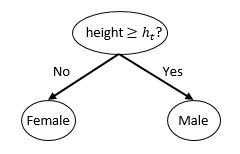
\includegraphics[width=0.5\linewidth]{Images/decision_stump.png}
    \caption[Beispiel eines Entscheidungsstumpfes]{Beispiel eines Entscheidungsstumpfes (Quelle: Sefik Ilkin Serengil, sefiks.com)}
    \label{fig:decision_stump}
\end{figure}

% \subsection{Modern Approaches in Machine Learning}
% Überblick über aktuelle Trends und Innovationen im Machine Learning
% Vorstellung fortgeschrittener Techniken und Methoden
% Diskussion über die Bedeutung von Deep Learning und künstlichen neuronalen Netzen
% \subsection{Role of Boosting Algorithms in ML}
% Einführung in Boosting-Algorithmen und ihre Relevanz
% Spezifische Betrachtung von \gls{adaboost} und \gls{gradientboosting}
% Vergleich von Boosting-Algorithmen mit anderen fortgeschrittenen Methoden
% \subsection{Boosting Algorithms in Tabular Data Analysis}
% Bedeutung von tabellenartigen Datensätzen in fortgeschrittenen ML-Anwendungen
% Analyse, wie \gls{adaboost} und \gls{gradientboosting} bei tabellenartigen Daten effektiv sind
% Fallstudien und Beispiele aus der Praxis, die den Einsatz dieser Algorithmen zeigen

% Daten
% Entscheidungsbäume
% Traingsfehler
